%! Install TeXiFy IDEA plugin if you want to be able to properly edit .tex files in IntelliJ
%! (has code completion, etc.)

\documentclass[12pt,a4paper, oneside]{article}
\usepackage[utf8]{inputenc}
\usepackage[T1]{fontenc}
\usepackage[english,german]{babel}
\usepackage[style=german]{csquotes}
\usepackage{graphicx}

\author{Uni Oldenburg, SWP2020 Gruppe A}

\begin{document}

    \begin{titlepage}
        \pagestyle{empty}
        \begin{center}

            \begin{figure}[h]
                \centering
                
\includegraphics[width=0.35\textwidth]{../img/Logo.jpg}
            \end{figure}

            \bigskip \bigskip \noindent
            \textsc{\textbf{\LARGE Softwareprojekt:}} \par \bigskip \noindent
            \textsc{\textbf{\LARGE Projekttagebuch}}


            \par \bigskip \bigskip \bigskip \bigskip \bigskip \noindent
            {\Large Gruppe A} \par \medskip \noindent

            \par \bigskip \bigskip \bigskip \bigskip \bigskip \bigskip \noindent
            \textit{\Large Wintersemester 2020/21 und} \par \noindent
            \textit{\Large Sommersemester 2021}

            \par \bigskip \bigskip \bigskip \bigskip \bigskip \bigskip \noindent
            \par \bigskip \bigskip \bigskip \noindent
            {\Large Sprintanalyse} \par \medskip \noindent

        \end{center}
    \end{titlepage}

    \tableofcontents
    \pagebreak


    \section{Sprinttagebuch: Sprint-Nr. 9}
    \underline{Name des Sprints:}
    \\
    Sprint 9: Fear of the Dark

    \noindent
    \\
    \underline{Zeitraum des Sprints:}
    \\
    15. April 2021 - 04. Mai 2021

    \noindent
    \\
    \underline{Ziel des Sprints:}
    \\
    UX und Feinschliff

    \noindent
    \\
    \underline {Team:}
    \\
    Sven Ahrens, Alwin Bossert, Aldin Dervisi, Marvin Drees, Mario Fokken,
    Timo Gerken, Finn Haase, Temmo Junkhoff, Maximilian Lindner, Steven Luong,
    Phillip-André Suhr, Eric Vuong


    \section{Vorgänge}

    \begin{itemize}
        \item SWP2020A-131:	ANmi eine Hilfsanzeige für meine aktuellen Möglichkeiten haben (3 Story Points)

        \item SWP2020A-132:	Spieler soll eine Regelübersicht einsehen können (1 Story Points)

        \item SWP2020A-140:	ANmi, dass die Längste Handelsstraße und Größte Rittermacht automatisch korrekt zugewiesen werden (2 Story Points)

        \item SWP2020A-197:	ANmi die optionale Gründerphase zu Partiebeginn nutzen können (3 Story Points)

        \item SWP2020A-204:	ANmi, dass es eine maximale Zugzeit gibt, nach Ablauf derer "End Turn" vom System forciert wird (3 Story Points)

        \item SWP2020A-208:	ANmi im Lobbychat sehen können, wer der Lobby beigetreten bzw. sie verlassen hat (1 Story Points)

        \item SWP2020A-228:	ANmi eine Lobby mit einem Passwort schützen können, damit keine Fremden beitreten können (1 Story Points)

        \item SWP2020A-230:	ANmi sehen können, wie lange die aktuelle Partie bereits gespielt wird (1 Story Points)

        \item SWP2020A-234:	ANmi beim Bauen sehen können, an welchen Stellen ich (noch) bauen darf (2 Story Points)

        \item SWP2020A-245:	ANmi als Owner einer Lobby den Ownerstatus auf einen bestimmten Mitspieler übertragen können (1 Story Points)

        \item SWP2020A-246:	ANmi vor Start einer Partie durch Zufall die Zugreihenfolge bestimmen können (1 Story Points)

        \item SWP2020A-249:	Inventare als 2 TableViews (Ressourcen, Karten) umsetzen (Spalte für Anzahl und Spalte für Namen) (2 Story Points)

        \item SWP2020A-255:	Bericht für Sprint 08 erstellen (2 Story Points)

        \item SWP2020A-261:	ANmi in einer Partie sehen können, in welcher Runde sich das Spiel befindet (1 Story Points)

        \item SWP2020A-266:	TradeWith*Presenter abstrahieren (1 Story Points)

        \item SWP2020A-267:	Nach "Restart Lobby" werden bei anderen Teilnehmern noch die Ressourcenanzahlen in der Memberliste und der Systemnachrichtenverlauf im Chat angezeigt (2 Story Points)

        \item SWP2020A-268:	"Change Move Time"-Button und -Textfeld werden bei nicht-Ownern angezeigt (1 Story Points)

        \item SWP2020A-269:	"Confirm New Password"-Feld in ChangeAccountDetails einfügen (0 Story Points)

        \item SWP2020A-270:	Spielerzahleinstellung bei Lobbyerstellung rausnehmen & Standardwert auf 3 Spieler setzen (1 Story Points)

        \item SWP2020A-271:	AEmi das Loglevel in einer Configoption festlegen können (1 Story Points)

        \item SWP2020A-274:	Im Gameservice fehlen bei vielen Methoden Checks, ob die entsprechende Aktion überhaupt ausgeführt werden darf (2 Story Points)

        \item SWP2020A-277:	ANmi eine Option haben, damit automatisch gewürfelt wird (1 Story Points)

        \item SWP2020A-278:	AEmi Beschränkungen auf Nutzernamen und Lobbynamen haben (1 Story Points)

        \item SWP2020A-279:	Lobbybeitritt ist bereits auf dem "XYZ has won"-Screen möglich (1 Story Points)

        \item SWP2020A-281:	Redundantes setOnCloseRequest und window-Attribut im MainMenuPresenter entfernen (0 Story Points)

        \item SWP2020A-282:	Bereits vor dem Würfeln kann mit durch Anklicken eines Users mit ihm Resourcen tauschen (1 Story Points)

        \item SWP2020A-283:	Im serverseitigen Userservice muss die IllegalArgumentException vernünftig abgefangen werden (1 Story Points)

        \item SWP2020A-284:	UserServiceTest.registerSecondUserWithSameName (Server) ist erfolgreich, obwohl er korrekterweise eine Exception abfangen müsste (1 Story Points)

        \item SWP2020A-285:	Accountlöschung sollte eine Bestätigung erfordern (1 Story Points)

        \item SWP2020A-286:	ANmi die Straßenbaukarte mit ihrem Effekt nutzen können (2 Story Points)

        \item SWP2020A-288:	Passwort sollte bereits auf Clientseite gehasht werden, sodass es nur noch im Textfeld unverschlüsselt vorliegt (1 Story Points)

        \item SWP2020A-290:	ANmi über eine Configoption ein Theme auswählen können (3 Story Points)

        \item SWP2020A-295:	Turnindicator sollte Spielernamen in dessen Farbe anzeigen (0 Story Points)

        \item SWP2020A-296:	SessionManagementException im AuthenticationService wird nicht behandelt (0 Story Points)

        \item SWP2020A-297:	"java.io.IOException: Eine vorhandene Verbindung wurde vom Remotehost geschlossen" bei Serverabbruch braucht i18n (0 Story Points)

        \item SWP2020A-298:	Die AbstractX zwischen Interfaces und Implementierungen können entfernt werden (0 Story Points)

        \item SWP2020A-300:	Spielrelevante Buttons werden erst freigeschaltet, wenn alle Spieler mit dem Steuerbezahlen fertig sind (2 Story Points)

        \item SWP2020A-301:	SessionManagement kann nie die Session eines eingeloggten Nutzers finden und macht damit u.A. Handel kaputt (1 Story Points)

        \item SWP2020A-304:	LOG.isDebugEnabled() entfernen & LOG.debug-Formatting ausnutzen (0 Story Points)

        \item SWP2020A-305:	Bei Clientwechsel übernimmt die "Automatic Roll"-Checkbox nicht den vorherigen Zustand (0 Story Points)

        \item SWP2020A-309:	Beim Spielen einer Ritterkarte werden die spielrelevanten Buttons nicht disabled während der Räuber noch nicht neu platziert ist (1 Story Points)

        \item SWP2020A-310:	Monopolkarte nimmt anderen Spielern nicht alle Ressourcen der gewählten Sorte weg, sondern nur 1 & aktualisiert nicht die Inventare der bestohlenen Nutzer (0 Story Points)

        \item SWP2020A-311:	H2BasedUserStoreTest.getAllUsers schlägt in IntelliJ fehl (UserServiceTest sollte ein @AfterAll bekommen, das den dort verwendeten Nutzer entfernt) (0 Story Points)

        \item SWP2020A-223:	Diverse Klassen in Common aufteilen, um Zugriffsrechte einzuschränken & Enums verstärkt zu verwenden (3 Story Points)

    \end{itemize}

    \newpage

    \subsection{Sprinterfolg}

        \begin{figure}[h]
            \centering
            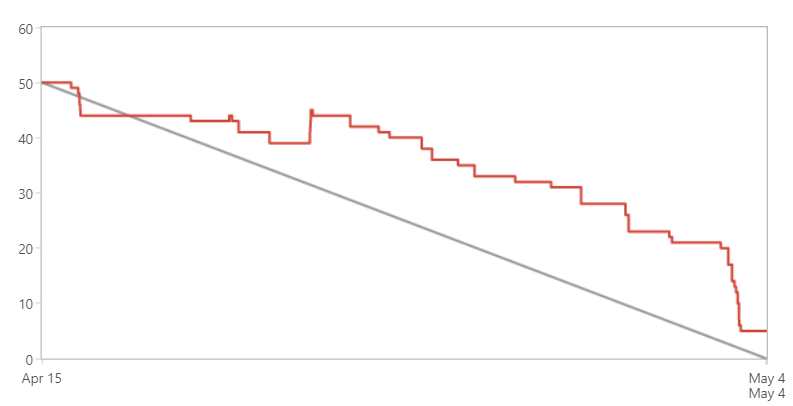
\includegraphics[width=\textwidth, height=5cm]{../img/sprint_09/Burndown-Sprint9.PNG}
            \caption{Burndown-Diagramm Sprint 9}
            \label{fig: Burndown-Sprint9}
        \end{figure}

        \noindent
        Dieser Sprint hatte im Gegensatz zum vorherigen 15 Story Points mehr zu beginn. Da der Spint hauptsächlich zur Verbesserung der UX und dem Feinschliff diente, waren die Tasks mit höchstens 3 Punkten bewertet, außerdem hatten einige sehr kleine Verbesserungen nur 0 Punkte.

    \subsection{Sprintprobleme bzw. Hindernisse}
    Wie man an dem Burndown-Diagramm erkennen kann, sind sehr viele Tasks erst kurz vor Ende des Sprints fertiggestellt worden, das führte dazu, dass es noch einige Mergekonflikte gab, die dann sehr schnell behoben werden mussten. Außerdem wurde die Task 223 nicht fertiggestellt und in den nächsten Sprint verschoben, da der Aufwand größer war als gedacht. Deshalb wurden die Story Points dieser Task von 3 auf 5 erhöht.

    \section{Erkenntnis aus der Retroperspektive}
    Folgende Erkenntnisse ergaben sich aus der Retrospektive:\\

    \underline{Start:}
    \begin{itemize}
        \item Entwurf/Ansatz nach 1 Woche bei Story mit 3+ Points
        \item Bei umfangreicheren Storys: Pair-Programming
        \item Recherche bei Verständnisproblemen
    \end{itemize}

    \underline{Stop:}
    \begin{itemize}
        \item Against popular belief: Bei den Reviews ist früher kommen besser
        \item Kummerkasten aktiv nutzen, damit wir dies Toll vermeiden können
    \end{itemize}

    \underline{Weiter so:}
    \begin{itemize}
        \item Bei kleineren Storys: Solo-Programming
        \item Weiterhin innerhalb von 36-48 Stunden auf Anschreiben reagieren
        \item Gründliche Reviews
    \end{itemize}

    \section{sonstige Anmerkungen}
%Falls es keine sonstigen Anmerkungen gibt, dann kann diese Sektion rausgelöscht werden.


    \section{Fazit}

\end{document}
